\documentclass[a4paper,11pt]{article}
\usepackage[utf8]{inputenc}
\usepackage[paper=a4paper, hmargin=1.5cm, bottom=1.5cm, top=3.5cm]{geometry}
\usepackage[T1]{fontenc}
\usepackage[spanish]{babel}
\usepackage[colorlinks=true, linkcolor=blue]{hyperref} %Links para el indice.
\usepackage{amsfonts}
\usepackage{verbatim}
\usepackage{listings}
\usepackage{caption}
\usepackage{subcaption}

\usepackage[section]{placeins}
\usepackage{float}
%\usepackage{adjustbox}
\usepackage{amsmath}
\usepackage{blindtext}
\usepackage{sidecap}
\usepackage{color}
\usepackage{graphicx}
\usepackage{algpseudocode}

% \newcommand{\real}{\hbox{\bf R}}

\newcommand{\funcName}[1]{\textbf{\texttt{#1}}}


\title{Trabajo Práctico de Sistemas Operativos}

\begin{document}

\maketitle

\begin{center}
	Universidad de Buenos Aires - Departamento de Computaci\'on - FCEN
\end{center}

\vspace{2cm}
Integrantes:

\begin{itemize}
	\item Castro, Dami\'an L.U.: 326/11  \verb+ltdicai@gmail.com+
	\item Toffoletti, Luis L.U.: 827/11 \verb+luis.toffoletti@gmail.com+
	\item Zanollo, Florencia L.U.: 934/11 \verb+florenciazanollo@gmail.com+
\end{itemize}

\newpage

\tableofcontents

\newpage

\section{Introducción}

Una computadora moderna consiste de uno o m\'as procesadores, memoria, discos, impresoras y uno o varios dispositivos de entrada/salida. Adem\'as una computadora ejecuta programas que suelen intentar acceder a estos recursos y generalmente asumiendo que son los \'unicos que desean utilizarlos. Sin embargo esto casi nunca es cierto y suelen haber conflictos cuando dos procesos (programas en ejecuci\'on) acceden al mismo recurso. Para solucionar estas problem\'aticas se recurre a los sistemas operativos, que son aquellos que se encargan de coordinar el acceso a los recursos por parte de los procesos. Un sistema operativo es un proceso superior a todos los dem\'as y decide, siguiendo alguna normativa, en que momentos los procesos comunes se ejecutan. Se conoce a esta normativa como pol\'itica de \emph{scheduling}, y no hay una \'unica manera de definirla. Dependiendo de la situaci\'on puede que se prefiera pol\'iticas que permitan a los procesos mantener ocupado un recurso durante per\'iodos largos de tiempo mientras que otras pol\'iticas se valen en desalojar a las tareas y otorgarle los recursos a otra tarea. Se espera que un \emph{scheduler} trate de cumplir los siguientes objetivos:

\begin{itemize}
	\item Ecuanimidad (\emph{fairness}): que cada proceso reciba una dosis “justa” de CPU (para alguna definici\'on de justicia).
	\item Eficiencia: tratar de que la CPU est\'e ocupada todo el tiempo.
	\item Carga del sistema: minimizar la cantidad de procesos listos que est\'an esperando CPU.
	\item Tiempo de respuesta: minimizar el tiempo de respuesta percibido por los usuarios interactivos.
	\item Latencia: minimizar el tiempo requerido para que un proceso empiece a dar resultados.
	\item Tiempo de ejecuci\'on: minimizar el tiempo total que le toma a un proceso ejecutar completamente.
	\item Rendimiento (throughput): maximizar el n\'umero de procesos terminados por unidad de tiempo.
	\item Liberaci\'on de recursos: hacer que terminen cuanto antes los procesos que tiene reservados m\'as recursos.
\end{itemize}

Como se puede intuir, es imposible cumplir todos los objetivos a la vez, por lo tanto las pol\'iticas de \emph{scheduling} tienen sus ventajas y sus desventajas. Es el enfoque de este informe exhibir dichas pol\'iticas, su implementaci\'on en lenguaje \emph{C++} y mostraremos sus pros y sus contras con ejemplos.

\subsection{Simulador}

Para analizar las diferentes pol\'iticas de \emph{scheduling} utilizamos un modelo de computadora simplificado que consiste en los siguientes componentes:

\begin{itemize}
	\item Un lote de programas a ejecutar.
	\item Uno o varios n\'ucleos (\emph{cores}) de procesamiento, que se encargar\'an de hacer los c\'omputos de los procesos.
	\item Un \'unico dispositivo de entrada y salida que todos los procesos pueden utilizar si lo desean.
\end{itemize}

\subsubsection{Acciones del simulador}

El simulador provee a los procesos con tres acciones posibles:

\begin{itemize}
	\item $uso\_CPU$(\emph{n}) que indica que el proceso utilizar\'a el CPU durante \emph{n} ciclos de reloj.
	\item $uso\_IO$(\emph{n}) que indica que el proceso utilizar\'a un recurso de entrada/salida durante $n$ ciclos de reloj. Durante este tiempo el proceso no utiliza al procesador, as\'i que el \emph{scheduler} es libre de utilizar ese tiempo en otra tarea.
	\item $return$ que indica que el proceso ya termin\'o su ejecuci\'on. El \emph{scheduler} debe realizar las acciones necesarias para desalojar al proceso.
\end{itemize}

\subsubsection{Definici\'on de \emph{schedulers}}

Un \emph{scheduler} v\'alido ofrece las siguientes funcionalidades:
\begin{itemize}
	\item \funcName{load(pid)}: Carga un proceso con n\'umero de identificaci\'on \funcName{pid}. 
	\item \funcName{unblock(pid)}: Se realiza cuando un proceso con n\'umero de identificaci\'on \funcName{pid} deja de utilizar un recurso de entrada/salida y desea volver a usar el procesador.
	\item \funcName{tick(cpu,motivo)}: Se ejecuta por cada $tick$ del reloj del procesador \funcName{cpu} y el \funcName{motivo} indica que sucedi\'o con el \'ultimo proceso que estaba en ejecuci\'on.
\end{itemize}


\section{Pol\'iticas de \emph{scheduling}}

%\input{fcfs.tex}

%\input{rr.tex}

%\subsection{Lottery Scheduling}

La idea detr\'as de $lottery$ $scheduling$\cite{SchedLottery} es aplicar un enfoque probabil\'istico y pseudoaleatorio a la hora de asignar recursos a las tareas. Para lograr esto se utiliza un sistema de $tickets$ que representan derechos de acceso a recursos; las tareas poseen una cantidad determinada de $tickets$, puediendo ser distinta de una tarea a otra y cada vez que el $scheduler$ decide a qu\'e tarea otorgar los recursos lo hace mediante una loter\'ia, elige uno entre todos los $tickets$ del sistema. El proceso que tenga ese $ticket$ ser\'a el ganador y se le asignar\'a el recurso que est\'a demandado.

Los $tickets$ son una forma de cuantificar los derechos de acceso a recursos; cuantos m\'as $tickets$ tenga una tarea, m\'as probable es que gane la loter\'ia. Tambi\'en permiten homogeneizar los diferentes tipos de recursos ya que todos son representados por los mismos tipos de $tickets$, esto aporta flexibilidad a la hora de asignarlos.

\subsubsection{Loter\'ias}

En cada $tick$ del reloj, el $scheduler$ toma una decisi\'on: si el proceso en ejecuci\'on agot\'o todo su quantum asignado, realiz\'o una llamada bloqueante o simplemente termin\'o exitosamente entonces se lleva a cabo una loter\'ia. Est\'a loter\'ia decide qui\'en va a ser el pr\'oximo proceso en utilizar el recurso deseado. Elegir el $ticket$ ganador se realiza mediante un algoritmo pseudoaleatorio que lo elige de manera uniforme, esto es, todos los tickets tienen una probabilidad igual de ganar la loter\'ia, a saber:

Sea $n$ la cantidad de $tickets$ y \{t$_i$\}$_{1 \leq i \leq n}$ el conjunto de ellos.

\[
	P(t_{i}) = \frac{1}{n}
\]

Luego, la probabilidad que un proceso $j$ que posee $t$ cantidad de $tickets$ gane la loter\'ia es igual a:


\[
	P(j \text{ gane la loter\'ia}) = \sum_{1}^{t}\frac{1}{n} = \frac{t}{n}
\]

Se puede probar que la cantidad de loter\'ias ganadas por la tarea $j$ sigue una distribuci\'on binomial de par\'ametro $p = \frac{t}{n}$. De esta manera se observa que la esperanza de la cantidad de loter\'ias ganadas por una tarea es igual a:

\[
	E(\text{cantidad de loter\'ias ganadas}) = \frac{t}{n}*\text{cantidad de loter\'ias realizadas}
\]

Esto implica que el valor promedio de la cantidad de loter\'ias ganadas es directamente proporcional a la cantidad de $tickets$ que posee la tarea. Por esta raz\'on se dice que $lottery$ $scheduling$ es probabil\'isticamente justo.

\subsubsection{Fairness}

\subsubsection{Compensation tickets}

Queremos ver cómo se comporta el algoritmo ante un lote de tareas compuesto por
tareas que sólo utilizan CPU y otras que realizan llamadas bloqueantes.\\

Si SchedLottery no contara con compensation tickets entonces como se explica en el artículo \cite[Sec. 3.4]{SchedLottery} el problema se 
ocasiona cuando una tarea se bloquea sin terminar de utilizar su quantum.
De continuar así por varios ciclos entonces esa tarea usaría, en promedio, menos CPU que las demás
(la probabilidad de ganar el sorteo es la misma para todas, pero en este caso habría tareas que
usan más tiempo el CPU que las demás)
violando así la regla de 1:1 dónde todas deberían recibir la misma proporción de CPU.\\

La forma propuesta para contrarrestar este problema es Compensation Tickets. 
Consiste en dar a la tarea bloqueada una cantidad de tickets en relación con el quantum no utilizado.
Así, si sólo utilizó una fracción $f$ del quantum le son dados $cant\_inicial/f$ tickets.\\

Queremos mostrar evidencia de que el sistema de compensation tickets (CT) corrige el problema
previamente mencionado sobre la asignación de CPU esperada entre tareas bloqueantes y no bloqueantes.
Para esto ejecutamos dos tareas, una taskBatch, ya que el problema se manifiesta cuando existen llamadas bloqueantes, y la otra taskCPU.\\

Al comienzo cada tarea posee 10 tickets (misma probabilidad de ganar) porque queremos que se ejecuten equitativamente.\\
Para mostrar que efectivamente hay una mejora en la distribución del CPU presentamos los datos mediante tablas, donde cada columna pertenece a un ciclo en particular 
y cada fila a una tarea.\\
Ej: La posición de la tabla fila x, columna y: tiene la cantidad de CPU utilizada por la tarea x hasta el ciclo y.\\

\begin{flushleft}
\textbf{SchedLottery sin CT:}\end{flushleft} %-------------------------------------------------------------------------------------------------------------

\begin{center}
 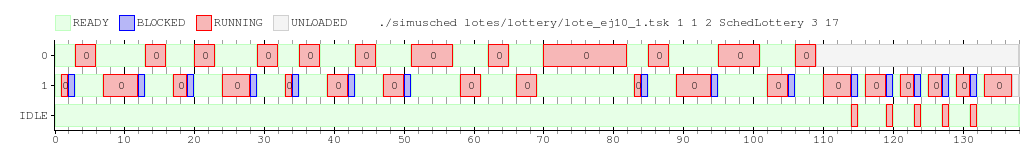
\includegraphics[scale=0.48]{./Lottery/ej10_SIN_CT.png}
\end{center}

\begin{center}
\begin{tabular}{|c|c|c|c|c|c|c|c|c|c|c|c|c|c|c|}
\hline
Ciclo & 10 & 20 & 30 & 40 & 50 & 60 & 70 & 80 & 90 & 100 & 110 & 120 & 130 & 137\\
\hline
\hline
Tarea 0 (CPU) & 3 & 6 & 10 & 15 & 18 & 24 & 27 & 37 & 42 & 47 & 51 & - & - & - \\
\hline
Tarea 1 (Batch) & 4 & 8 & 12 & 14 & 19 & 21 & 25 & 25 & 27 & 31 & 34 & 41 & 46 & 51 \\
\hline
\end{tabular}\end{center}

Hasta el ciclo 80 el CPU se mantiene relativamente distribuido. Luego la tarea 0 pasa a tener mayor proporción hasta que finaliza. 
Si esto se proyecta en el tiempo entonces la brecha se vuelve cada vez más grande.

\begin{flushleft}
\textbf{SchedLottery con CT:}\end{flushleft} %--------------------------------------------------------------------------------------------------------------

\begin{center}
 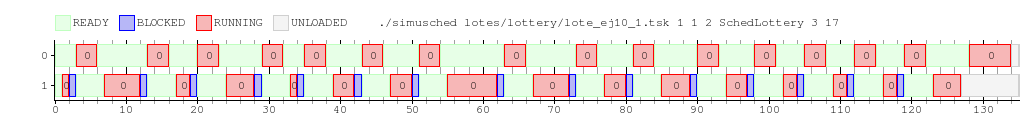
\includegraphics[scale=0.48]{./Lottery/ej10_CON_CT.png}
\end{center}

\begin{center}
\begin{tabular}{|c|c|c|c|c|c|c|c|c|c|c|c|c|c|c|}
\hline
Ciclo & 10 & 20 & 30 & 40 & 50 & 60 & 70 & 80 & 90 & 100 & 110 & 120 & 130 & 134 \\
\hline
\hline
Tarea 0 (CPU) & 3 & 6 & 10 & 15 & 18 & 21 & 24 & 27 & 30 & 35 & 39 & 43 & 47 & 51\\
\hline
Tarea 1 (Batch) & 4 & 8 & 12 & 14 & 19 & 24 & 29 & 34 & 38 & 41 & 44 & 47 & 51 & -\\
\hline
\end{tabular}\end{center}



\section{Discusi\'on}

\section{Conclusiones}


\end{document}
